\chapter{Empathy for a toy robot with a story}
\label{chap_hexbug}

\section{Summary}

To test if implicit life-stories of robots evoke our empathy, I conducted a human subject study where participants were asked to strike a robot with a life-story. From analysis of participant's hesitation to inflict harm and from psycometric tests, I found that stories can engender empathy for robots.



   \begin{figure}[thpb]
      \centering
      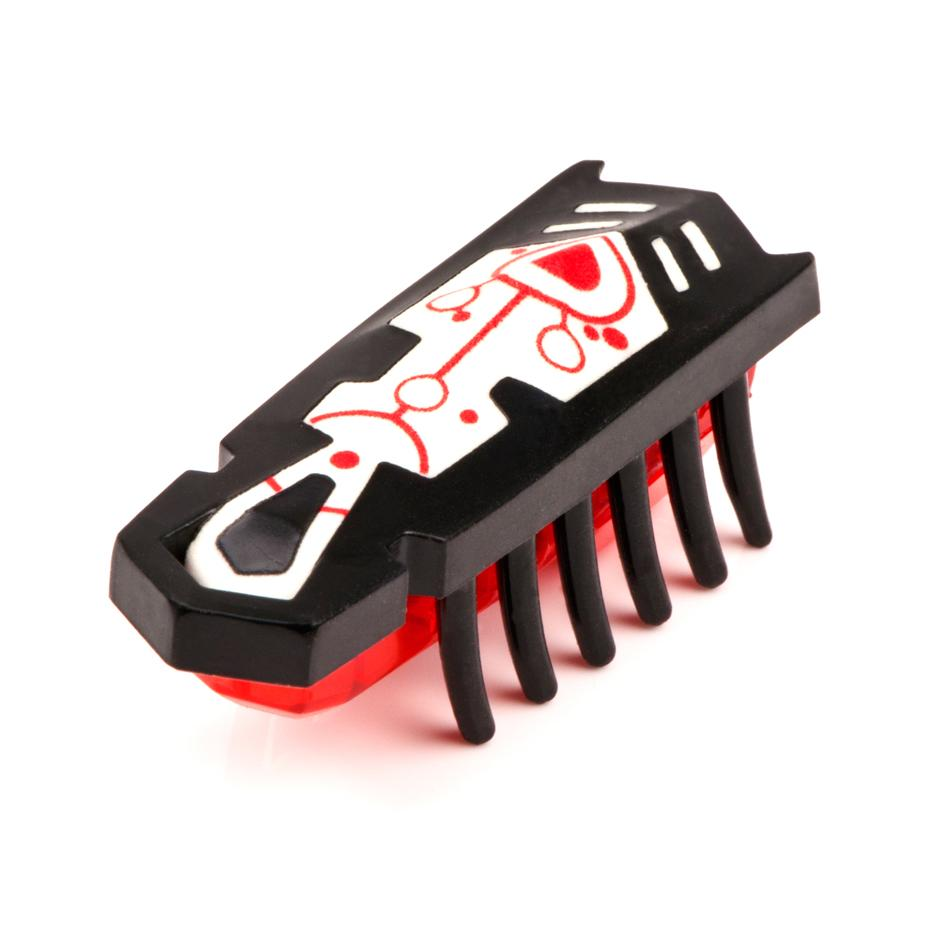
\includegraphics[width=2.2in]{figures/hexbug/hexbug_nano.jpg}
      \caption{Hexbug Nano toy robot used in the study described here.}
      \label{fig_hexbug_hexbug_nano}
   \end{figure}


\section{Study Design}

I conducted this study with Kate Darling, a research specialist also at the Media Lab \cite{darling_hexbug_study}. Along with implict life-stories, we were interested in testing if personified life-stories and movement had impact on empathy. 

Empathy is an internal state so it isn't possible to directly measure empathy.
However, we reasoned that if people feel empathy towards a robot they will not want to harm it. If empathy is the cause for hesitation, then it also stands to reason that those with greater tendency to empathize with others, ie. trait empathy, would empathize with the robot more and consequently would hesitate more. Accordingly, we also evaluated teh relationship between hesitation to strike a robot and the participant's trait empathy.


\section{Method}
To test our hypotheses, we conducted a between subjects experiment with six conditions (3x2). Because we were interested in the effect of movement and two different stories, the six conditions are the cross product of two factors, one with two levels (movement, no movement) and the other with three levels (no story, personified story, implicit life-story). For this thesis, I will focus mostly on the implicit life-story condition. In the experiment, participants were asked to observe a Hexbug Nano, a small robotic toy (Figure \ref{fig_hexbug_hexbug_nano} ), and then strike it with a mallet.

In order to assess subjects' trait empathy, we used the Interpersonal Reactivity Index and measured subjects' scores on the three subscales fantasy, empathic concern, and personal distress described earlier in Chapter 2. Given the limited nature of the Hexbug robot, we omitted the highly cognitive subscale of perspective taking in the interest of brevity. 

\subsection{Hypotheses}

H1: \emph{Hesitation to strike a robot will be greater for robots that have a backstory describing the robot's prior experiences, as opposed to robots with no story.}

H2: \emph{Hesitation to strike a robot will be greater for subjects with high trait empathy scores, as opposed to subjects with low trait empathy scores.}

H3: \emph{The effect of stories on hesitation will be more pronounced for subjects with high trait empathy scores, as opposed to subjects with low trait empathy scores.}

\subsection{Participants}


A group of 101 subjects recruited via university mailing lists participated in the experiment. Of the subjects, 48 self-identified as female, 52 as male, and 1 as other. The age range was 18-57 years old ($\mu=29, sd=9.7$). Subjects were randomly assigned to one of the 6 conditions resulting in 16-18 subjects per condition. The subjects were given a Hexbug Nano for their time and participation. 


\subsection{Experiment Setting and Conditions}

   \begin{figure}[thpb]
      \centering
      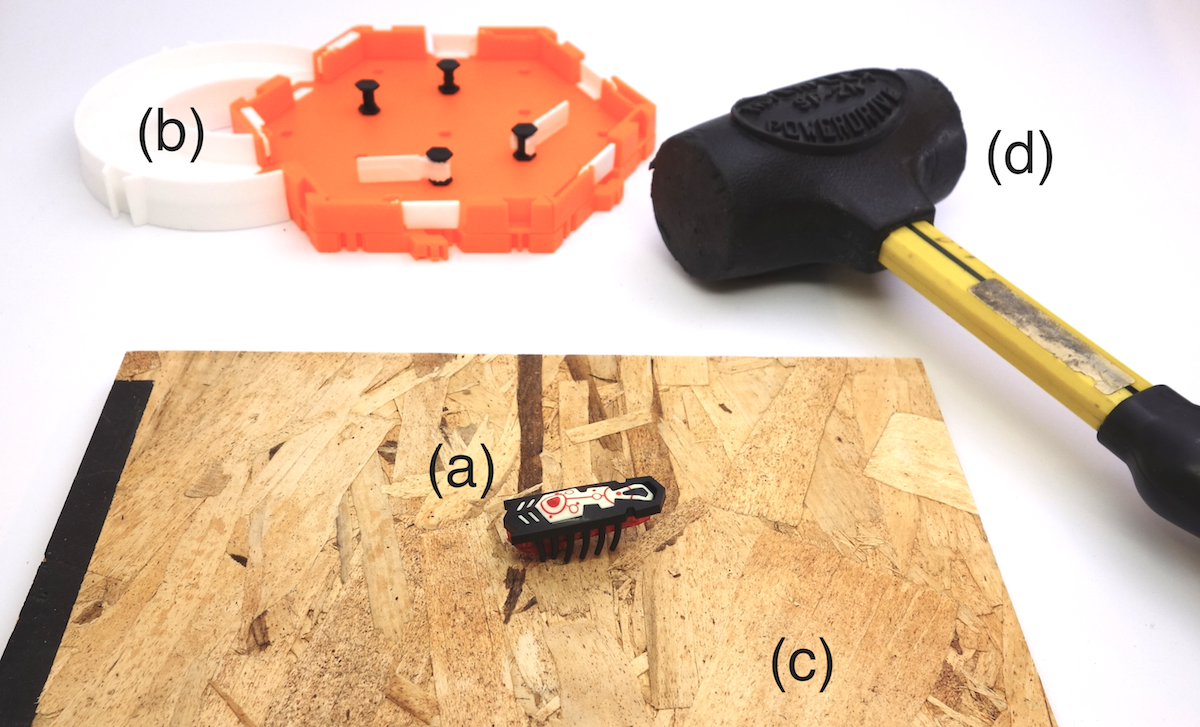
\includegraphics[width=4.6in]{figures/hexbug/setup_small.png}
      \caption{Experiment Materials: (a) Hexbug Nano, (b) Confined space for movement, (c) Board with hidden magnet for immobilizing Hexbug, (d) Mallet}
      \label{experiment_setup}
   \end{figure}

The subjects were informed that they were participating in a human robot interaction study but did not know they would be asked to strike a robot. Sessions in the experiment area were videotaped. The robot was on a table confined within a partition where it was able to move around. There was a mallet in the room concealed from the subjects' view. Subjects were reminded that they may stop the study at any time.
 
In the control condition (non-movement, non-story), the experimenter asked the subjects to observe a motionless Hexbug in the partition. After this, the experimenter moved the Hexbug to a board on the same table (onto a magnet that held it in place, allowing for easy aim). Then the experimenter revealed the mallet, placed it in the subject's dominant hand, and instructed the subject to ``strike the object with the mallet.'' 

In the movement conditions, subjects first observed a moving Hexbug and were then similarly instructed to ``strike the object with the mallet.''
 
In the story conditions, the subjects first observed a moving or non-moving Hexbug and were then given a text on a piece of paper to read. For the personification story, they were given the following text: \emph{``This is Frank. Frank is really friendly but he gets distracted easily. He's lived at the Lab for a few months now. He likes to play and run around. Sometimes he escapes, but he never gets far. Frank's favorite color is red. Last week, he played with some other bugs and he's been excited ever since.''} Keeping in line with the personification element of the story, the subjects were then instructed to strike ``Frank'' with the mallet.
 
For the experience story, subjects were given the following text: \emph{``This object has been around the Lab for a few months now. If you had come by before, you would have seen it moving around on the floor. It gets around but doesn't go too far from the lab. Last week though, it got out of the building and has been behaving oddly ever since.''} The subjects were then instructed to ``strike the object with the mallet.''


The experiment was over once the subject followed the instruction and struck the Hexbug or did not comply.


Post-experiment, the subjects were asked to fill out a survey, including the empathy test. Because the Interpersonal Reactivity Index measures trait empathy, administering the test after the experiment is not assumed to have an effect on subjects'’ scores.
 
\subsection{Measures}


We timed the relative hesitation or refusal of the subjects to strike the Hexbug as the main dependent variable. We measured hesitation time as the interval between the end of the instructions to the time the subject struck. If the subject asked a question indicating they had not understood what they had been instructed to do (e.g. ``Did you say you want me to track it?'', not ``Will it hurt him?''), we took the time interval from the end of the experimenter's answer to the strike time as hesitation time. The time was coded from the captured video session. If the subject asked a question, the time was then coded by two independent coders (Krippendorff's $\alpha=0.96$). We took the mean of the two coded times as the hesitation time. 
If a subject did not strike the robot, we considered this to be greater hesitation than the maximum measured hesitation and set the value at 1 second more than the maximum. The rank-based tests in the analysis are not affected by any particular value for the difference as long as it is positive. 

We also asked participants to fill out a post-experiment survey to capture a self-assessment of reasons for hesitation, and basic demographical information, as well as the three subscales of the Interpersonal Reactivity Index.  

\section{Results}
 \subsection{Hesitation}

We analyzed the measured hesitation across conditions. We first tested for normality of the distribution using the Shapiro Wilk test. The hypothesis that the data was normal was rejected ($p < 0.001$), so we analyzed the data using non-parametric ranked based tests (Mann-Whitney, Spearman and ranked ANOVA). 



% they had suggested wrapping the graphics with \framebox for morestability.

   \begin{figure}[thpb]
      \centering
      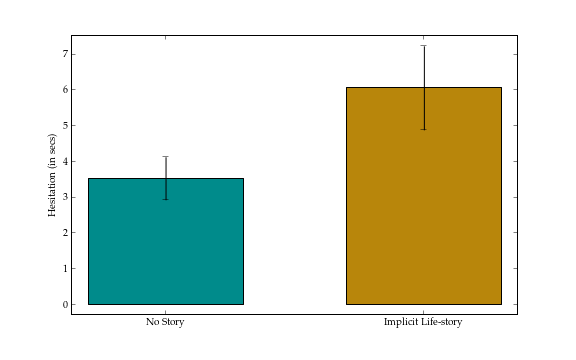
\includegraphics[width=4.6in]{figures/hexbug/story_hesitation.png}
      \caption{Mean hesitation (in secs) of implicit life-story vs no story conditions across all movement conditions. Error bars show SD of mean.}
      \label{fig_story_hesitation}
   \end{figure}
   



We tested our hypotheses that story condition will increase hesitation using 1-tailed Mann-Whitney tests.  We found that subjects hesitated significantly longer for the life-story story condition compared to the non-story condition (H1) ($\mu_{experience}=6.06s, \mu_{non\_story}=3.53s, U=440.5, p<0.047$) (Fig. \ref{fig_story_hesitation}). There was no significant difference between the implicit life-story and personified stories or between the movement conditions.



In post-hoc analysis, we examined the interaction of the story and the movement factors. The greatest hesitation difference between story and non-story occurs when the object is not moving (Fig. \ref{fig_story_type_interaction}). Movement attenuates the effect of stories while increasing the hesitation for non-story conditions. There was no significant difference between the two story conditions in either of the movement conditions. We combined the four story conditions into two (movement and non-movement stories) to increase power and clarity of our analysis (Fig. \ref{fig_has_story_interaction}).



   \begin{figure}[thpb]
      \centering
      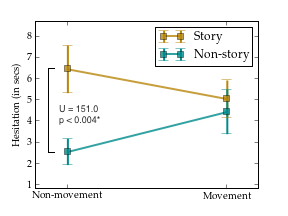
\includegraphics[width=4in]{figures/hexbug/has_story_interaction.png}
      \caption{Interaction of movement x story conditions showing mean hesitation and SD of mean.}
      \label{fig_has_story_interaction}
   \end{figure}
   





Four comparisons of hesitation are of interest: movement vs. non-movement for each of the two story conditions, as well as story vs. non-story for each of the two movement conditions. The results, summarized in Table \ref{table_has_story}, show that there is significant difference in the measured hesitation between story and non-story condition for the non-movement case ($\mu_{story}= 6.45s, \mu_{non\_story}=2.58s; U=151.0, p <0.004$; significant at $\alpha=0.05$ after Bonferroni correction for 4 comparisons). We will return to these results in the discussion section.



\begin{table}
\renewcommand{\arraystretch}{1.3}
\caption{Mean hesitation for Story X Movement}
\label{table_has_story}
\centering
\begin{tabular}{c||c|c|c}
\hline
& Story & Non-story & \specialcell{Mann Whitney\\ U, p}\\
\hline\hline

Movement & 5.05s & 4.44s & \specialcell{$U=281.5$,\\$p<0.384$} \\
\hline
Non-movement & 6.45s & 2.58s & \specialcell{$U=151.0$,\\$p<0.004$*}\\
%\footnote{is this in the table}}\\  %FIXME <--- get damn footnotes to work.
\hline
Mann Whitney U, p & \specialcell{$U=437.5$,\\$p<0.086$} & \specialcell{$U=124.5$,\\$p<0.178$} \\

\hline
\end{tabular}
\end{table}


\subsection{Empathy}


We had hypothesized that subjects with higher trait empathy would hesitate longer in striking the hexbug. (H2) We divided subjects into two equal sized groups of high and low empathy around the median value for each empathy subscale. Of the three subscales, we found  that those with high scores on empathic concern (EC)  hesitated significantly longer ($\mu_{high-EC}=6.39s, \mu_{low-EC}=3.55s; U=900.0, p<0.005;$ significant at $\alpha=0.05$ after Bonferroni correction for 3 comparisons). The other subscales Fantasy (FS) and Personal Distress (PD) do not show any significant changes in hesitation (Table \ref{table_empathy}).

 
\begin{table}
\renewcommand{\arraystretch}{1.3}
\caption{Mean hesitations for high and low empathy subjects for empathy subscales}
\label{table_empathy}
\centering
\begin{tabular}{c||c|c|c}
\hline
IRI Subscale & High Empathy & Low empathy & Mann-Whitney U, p\\
\hline\hline
FS & 5.59s & 4.33s & \specialcell{$U=1230.5$\\,$p<0.385$} \\
\hline
EC &  6.39s & 3.55s & \specialcell{$U=900.0$,\\$p<0.005*$} \\
\hline
PD & 5.56s & 4.26s & \specialcell{$U=1160.5$,\\$p<0.249$} \\
\hline
\end{tabular}
\end{table}



   \begin{figure}[thpb]
      \centering
      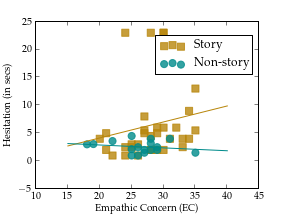
\includegraphics[width=4in]{figures/hexbug/ec_story_no_story_lm.png}
      \caption{Scatter plot of hesitation versus EC for non-movement data colored by story condition. Approximate regression lines are shown for illustrating difference in relationship between EC and hesitation for the story and non-story conditions. }
      \label{fig_ec_story_no_story_lm}
   \end{figure}
   

For the rest of the empathy analysis we look at just the two non-moving conditions (story vs non-story) where we see the greatest difference in the measured interaction. EC is moderately correlated with hesitation in the story condition (Spearman's $\rho=0.37$)  but weakly negatively correlated  (Spearman's $\rho=-0.12$) in the non-story condition (Fig. \ref{fig_ec_story_no_story_lm}).

To understand the effect of interaction of stories with empathic concern, we performed a two-way ANOVA-on-ranks test with Has-Story (Story and Non-Story) and EC as the independent variables and rank-transformed hesitation as the dependent variable. ANOVA-on-ranks showed a significant main effect of has-story ($F(1, 49)=8.92, p < 0.005$) and significant interaction of EC with Has-Story ($F(1, 47)=4.315, p < 0.044$). The significant interaction of EC with story holds even if we consider just the implicit life-stories ($F(1, 31) = 4.20, p < 0.05$)

We found no significant gender effect on subjects' hesitation to strike the robots.

\section{Discussion}
\label{sec_hexbug_discussion}

We hypothesized that hesitation to strike the robots would be greater for implicit life-story conditions compared to non-story conditions (H1). Our results confirm that stories can have an impact on people's reactions to robots. 

Interestingly, we noticed no significant difference in hesitation due to movement. We saw the greatest difference in hesitation between story and non-story for non-moving robots, but the difference became insignificant in the moving case (Fig. \ref{fig_has_story_interaction} ) We have two potential explanations for this. First, we could have been measuring two different types of reactions, depending on whether a subject has a strong aversion to insects or not. Some of the responses in our survey mentioned a dislike for cockroaches or bugs. Because subjects perceived the Hexbug as very insect-like, it is possible that people with low tolerance for insect-like movement reacted differently than people with high tolerance, creating conflicting effects. However, Fig. 3 indicates that there may be a more interesting relationship between story and movement. Another potential explanation is a disappointment of the subjects' behavioral expectations of the robot. Paepcke and Takayama have demonstrated that setting people's expectations low rather than high for a robot's competence leads to less disappointment and more positive evaluation of the robot \cite{paepcke_robot_low_expectations}. Because the Hexbug movements are very simple, it is possible that there was a disconnect between what the subjects believed the robot to be capable of based on our stories, and the behavior of the moving robot they were observing. I will re-examine this effect in when I discuss results from the final study in Chapter X. 

Consistent with our second hypothesis, we showed that those with high empathic concern hesitated more in striking the robot. (H2) This suggests that subjects' hesitation was a result of empathy for the robot. Prior studies in this area have had difficulty distinguishing between emotional hesitation and subjects hesitating for other reasons, for example because they did not want to damage something of perceived value. In our study, if the perceived value of the robot was greater for our moving or story conditions (because people attributed more intelligence or technical sophistication to the robot), this could have led to a similar hesitation effect. However, the fact that we find subjects with greater tendency for empathic concern hesitated more suggests that at least empathy is implicated in the hesitation.

Furthermore, for non-moving robots, we found a positive correlation between empathy and hesitation in the story condition and weak negative correlation for the non-story condition. Moreover, our analysis shows that there is significant interaction between empathic concern and stories on hesitation. These findings support our hypothesis that the effect of stories on hesitation is more pronounced for subjects with high trait empathy scores, as opposed to low (H3). This suggests that stories engender empathy, which results in hesitation. Adding descriptive color to our analysis, one question in our post-experiment survey asked subjects to describe in their own words why they hesitated. Many of our subjects used empathic terms to explain their hesitation, for example ``I had sympathy with him after reading his profile because I am also here in the Lab for a few month. [\emph{sic}]''

A study conducted by Rosenthal-von der P{\"u}tten et al., in which subjects watched videos of robots, showed a correlation between subjects' fantasy scores and their responses to the robots being mistreated \cite{rosenthal_emotional_reaction}. While this study may not be directly comparable to ours in many aspects, it is interesting that our study finds subjects' behavior to correlate with empathic concern, rather than fantasy. The fact that our subjects fell into a different category on the Interpersonal Reactivity Index indicates that we could be dealing with a different type of empathy. Further research may prove to support the suggestion that there is a divide between virtual and physical in how humans perceive and respond to robots \cite{bainbridge_robot_presence}, and also that emotional reactions to physical robots are not just guided by fantasy and imagination.


% momentum quote: “It's not who you think you are that holds you back it's who you think you're not.”


